\section{Problem Formulation}

\subsection{Wind Gradient Model}

As mentioned above in the background section, wind gradients can be generalized as a form of the power law, which has the following relationship:
\begin{equation}
    v_z = v_{ref} * (\frac{z}{z_{ref}})^{\alpha}  
    \label{eq:power_law}
\end{equation}

Equation~\ref{eq:power_law} follows a logarithmic relationship between the wind speed and altitude given some reference wind speed and altitude.
To abstract this into a more general form, where we dont need a reference wind speed and altitude this paper will be using the following equation for the wind gradient:
\begin{equation}
    v_{wind} (h) = a * ln(h + b)
    \label{eq:wind_gradient}
\end{equation}

Where $a$ and $b$ are constants the define the slope profile of the wind gradient. This translates to a function of $h$, the height above the ground.
Given a $h$, this returns the magnitude of the wind speed at that given height. Given a series of measurements of the wind at different heights, we can work to estimate the constants $a$ and $b$.
This allows us to estimate the wind gradient at any given height.

The large variety of wind gradients this relationship is able to capture is shown in Figure~\ref{fig:wind_gradients}.
As you can see, depending on the values of $a$ and $b$, a power law relationship can be created.

\begin{figure}[h]
    \centering
    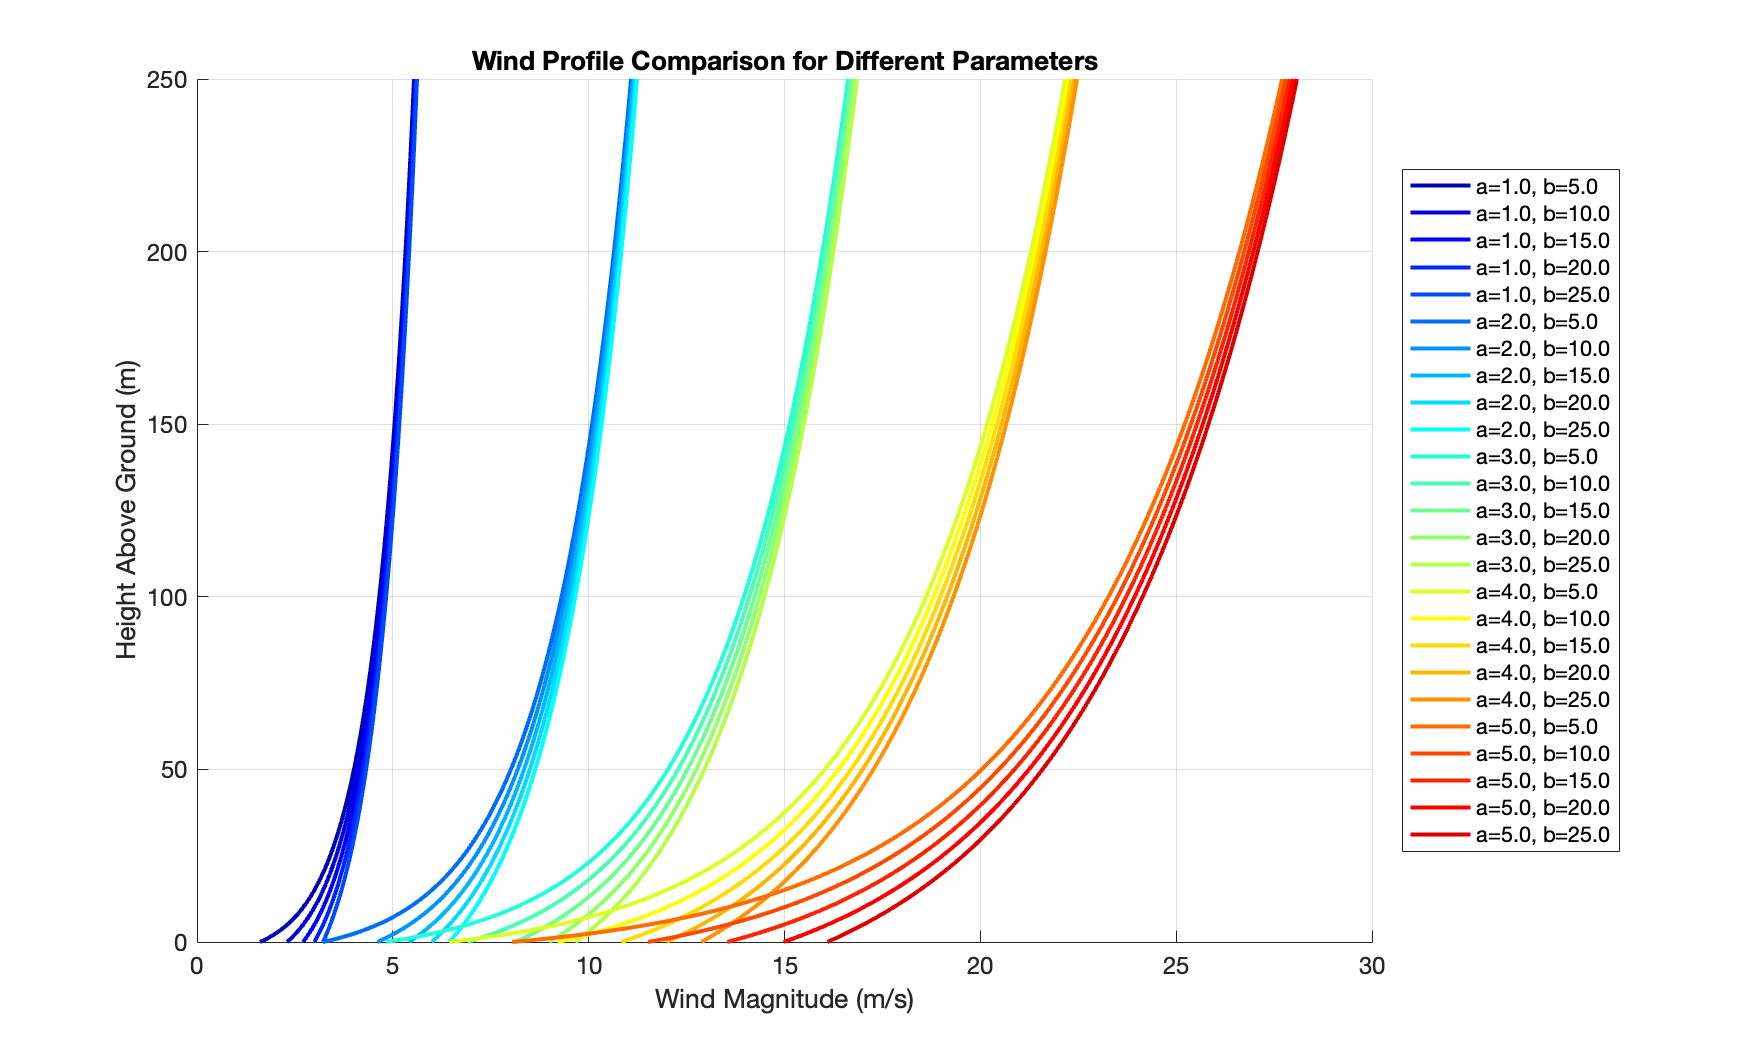
\includegraphics[width=0.6\textwidth]{images/wind_grads.png}
    \caption{Various wind gradient profiles. Comapring a and b values.}
    \label{fig:wind_gradients}
\end{figure}

\subsection{UAS Guidance Algorithm}

To measure the wind gradient, we will be using a series of UAS. These UAS will be flying a variety of straight line missions, each probing wind estimates from a different altitude. 
In order to command the UAS to follow a straight line mission, we will be using the lookahead straight line following algorithm, as given in Algorithm~\ref{alg:lookahead}.

\begin{algorithm}
    \caption{Lookahead Straight Line Following Guidance}\label{alg:lookahead}
    \begin{algorithmic}
    \State \textit{Given a current position, a line to follow (initial point and vector), and a lookhead distance, return the desired heading and velocity vector.}
    \Function{lookahead}{pos, line0, lineVec, lookahead}
    \State Calculate unit vector along line: $\hat{v} = \frac{lineVec}{||lineVec||}$
    \State Get rel pos of current to line start: $p_c = pos - line0$
    \State Project $p_c$ onto line: $p_{proj} = p_c \cdot \hat{v}$
    \State Get lookahead point: $p_{target} = line0 + (p_{proj} + lookahead) \cdot \hat{v}$
    \State Get error vector: $e = p_{target} - pos$
    \State Calculate desired heading: $\psi_d = \text{atan2}(e.y, e.x)$
    \State Calculate desired velocity vector: $v_d = \frac{e}{||e||} * ||lineVec||$
    \State Return heading and velocity vector
    \EndFunction
    \end{algorithmic}
\end{algorithm}

An image showing the visual trigonometry of the lookahead guidance algorithm for finding the target waypoint is shown in Figure~\ref{fig:lookahead}.

\begin{figure}[h]  
    \centering
    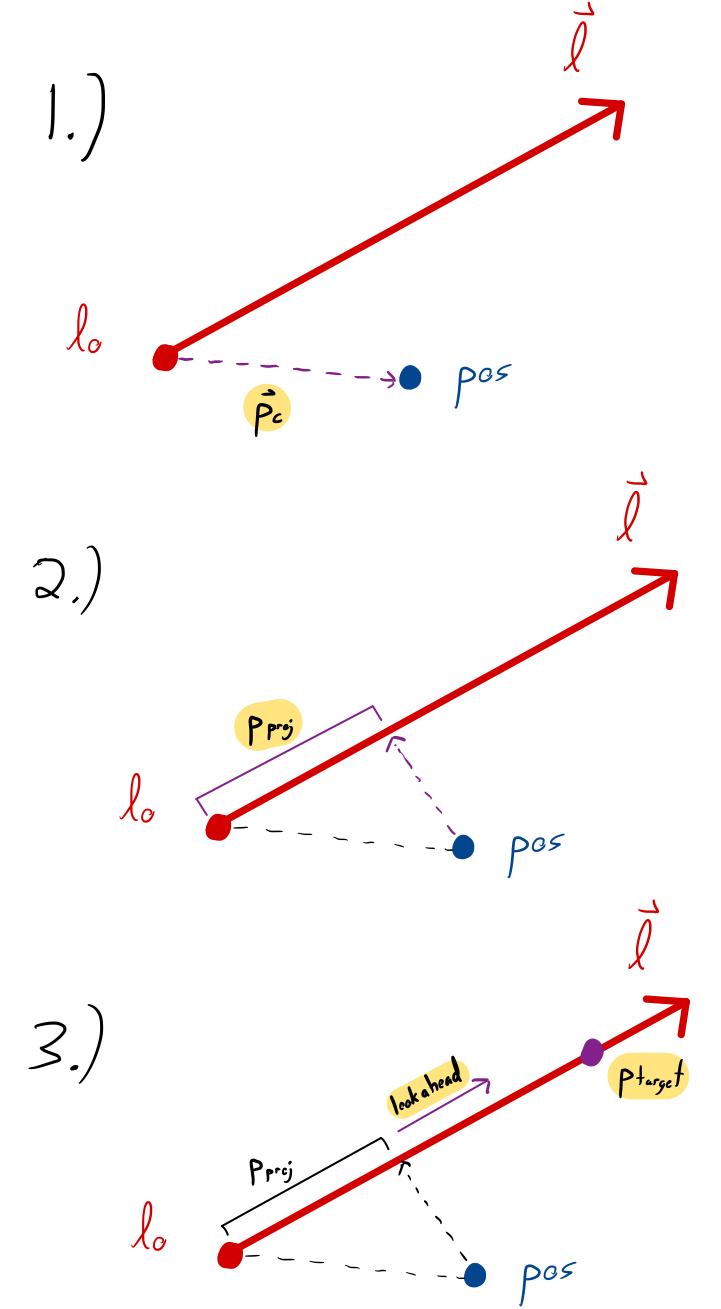
\includegraphics[width=0.35\textwidth]{images/proj_math.jpeg}
    \caption{Lookahead Guidance Trigonometry}
    \label{fig:lookahead}
\end{figure}

The autopilot a UAS uses is able to take in a desired heading, a desired height, and a desired height rate.
By taking these values from the lookahead guidance algorithm and simulating the UAS as a point mass through the vector field, through MATLAB's ode45, we get the result shown in Figure~\ref{fig:lookahead_sim} for a point mass following a guidance line:

\begin{figure}[h]  
    \centering
    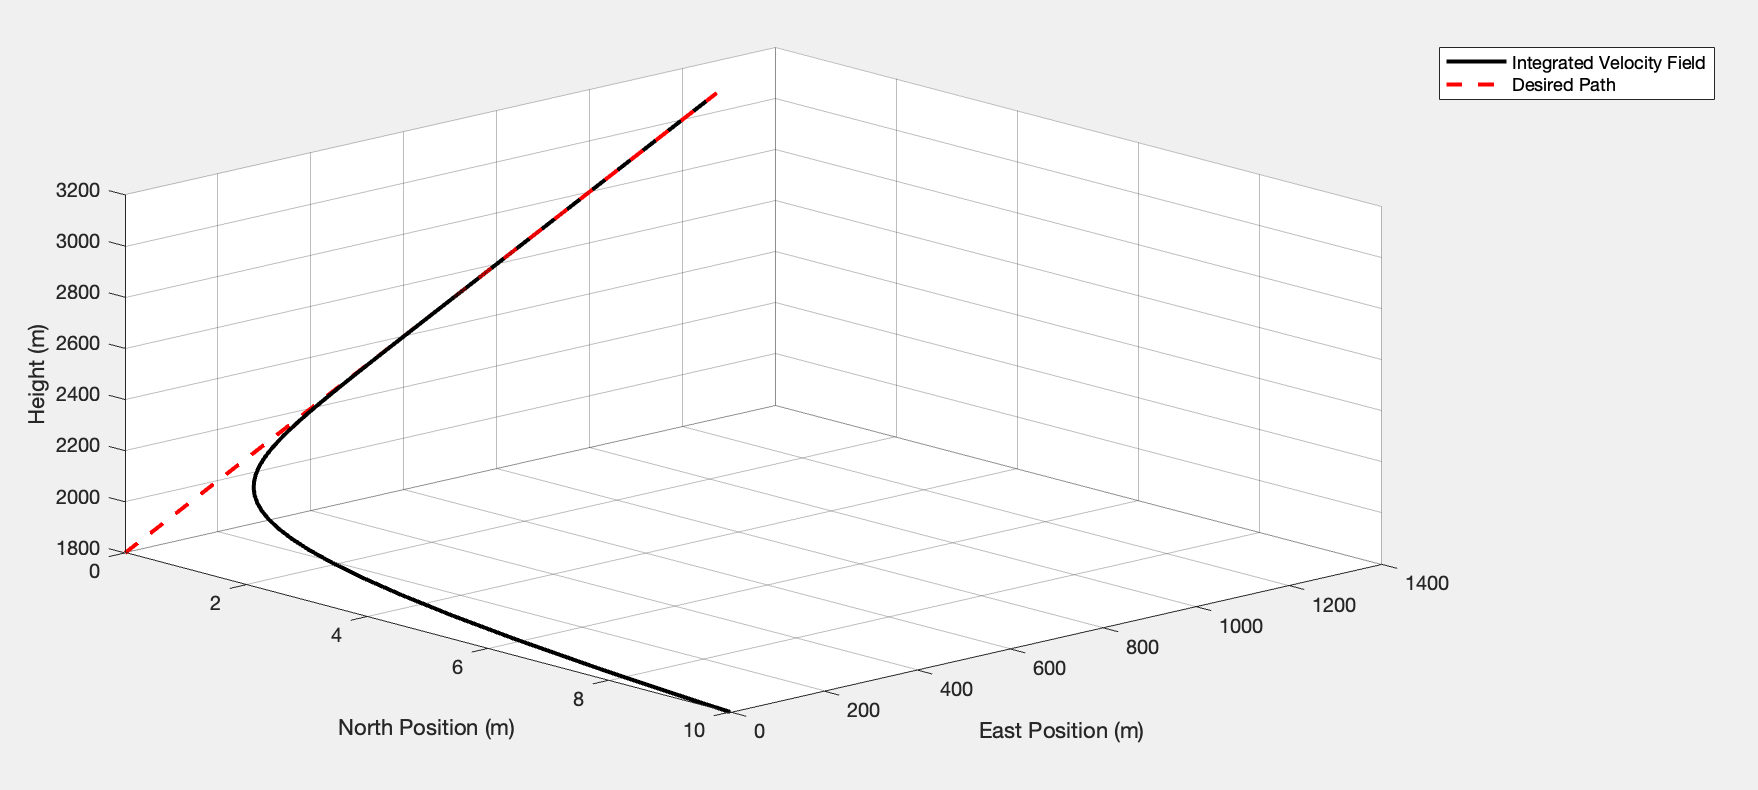
\includegraphics[width=0.5\textwidth]{images/lookahead_point.jpeg}
    \caption{Lookahead Guidance Simulation. Assuming point mass kinematics.}
    \label{fig:lookahead_sim}
\end{figure}

Thus, if the autopilot is able to correctly control based on desired heading, desired height, and desired height rate, we can command a UAS to follow a guidance line.

\subsection{UAS Autopilot Model}

The autopilot each UAS will be using is a successful loop closure controller, simulated in MATLAB.
The control block diagram for both the lateral and longitudal autopilot are shown in Figures~\ref{fig:lateral_autopilot} and~\ref{fig:longitudal_autopilot}, respectively.

\begin{figure}[h]  
    \centering
    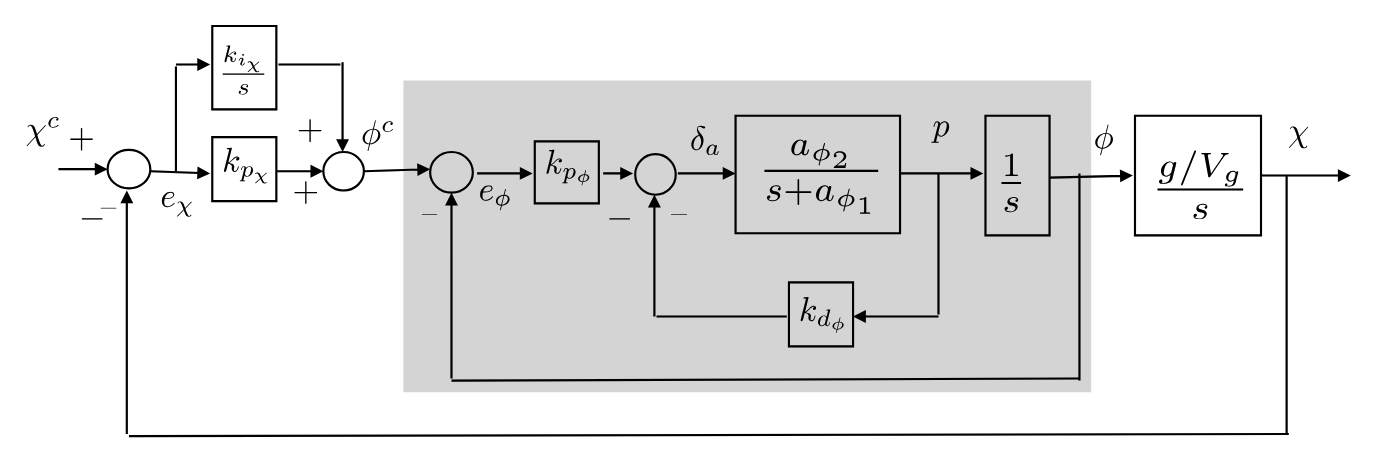
\includegraphics[width=0.5\textwidth]{images/lateral_auto.png}
    \caption{Lateral Autopilot Control Block Diagram}
    \label{fig:lateral_autopilot}
\end{figure}

\begin{figure}[h]  
    \centering
    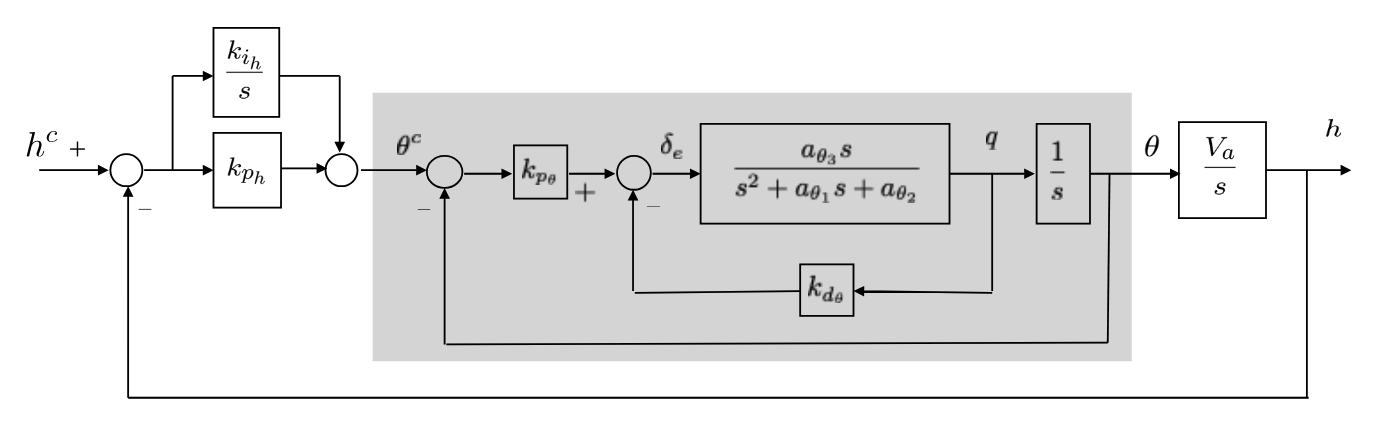
\includegraphics[width=0.5\textwidth]{images/long_auto.png}
    \caption{Longitudal Autopilot Control Block Diagram}
    \label{fig:longitudal_autopilot}
\end{figure}

In the lateral autopilot, the input is a desired heading, effecting the x and y position of the UAS.
In the longitudal autopilot, the input is a desired height, effecting the z position of the UAS.
For both of these autopilot systems, we will be using the successive loop closure (SLC) technique. 
The inner loops are shaded in gray, and by adjusting the gain values accordingly, we can assume that the inner loops react fast enough to be considered approximately perfect.
Thus, the outer loop can control heading and height, the high level commands, with the assumption the inner loop actuators and response are fast enough to be considered perfect.
The lookahead straight line following guidance algorithm given above outputs the heading and height desired at each iteration. 
This will be the guidance-autopilot loop used for all UAS in this paper.

\subsection{State and Wind Estimation}

In order to simulate using sensors to estimate the UAS's state and also the external wind, we will be using a combination of Extended Kalman Filters (EKFs) and low pass filters.
The state of a UAS is given by the vector:
\begin{equation}
    \mathbf{x} = \begin{bmatrix}
        \mathbf{x_E} \\
        \mathbf{y_E} \\
        \mathbf{z_E} \\
        \mathbf{\phi} \\
        \mathbf{\theta} \\
        \mathbf{\psi} \\
        \mathbf{u^{E}} \\
        \mathbf{v^{E}} \\
        \mathbf{w^{E}} \\
        \mathbf{p} \\
        \mathbf{q} \\
        \mathbf{r}\\
    \end{bmatrix}
\end{equation}

The tuple $\mathbf{x_E}, \mathbf{y_E}, \mathbf{z_E}$ is the position of the UAS in the inertial frame (north, east, down).
The tuple $\mathbf{\phi}, \mathbf{\theta}, \mathbf{\psi}$ is the euler angles for the attitude of the UAS (roll, pitch, yaw).
The tuple $\mathbf{u^{E}}, \mathbf{v^{E}}, \mathbf{w^{E}}$ is the inertial velocity in the UAS body frame (forward, right wing, down).
The tuple $\mathbf{p}, \mathbf{q}, \mathbf{r}$ is the angular velocity vector in the UAS body frame.

The position of the UAS is measured using a GPS sensor. The euler angles and angular rates are measured using a 3-axis rate gyroscope.

A low pass filter uses the following equation to filter measurements:
\begin{equation}
    \mathbf{y}_{new} = \alpha \mathbf{y}_{old} + (1 - \alpha) \mathbf{y}_{meas}
    \label{eq:low_pass}
\end{equation}

Where $\alpha$ maps to the equation $\alpha = e^{-a T_s}$. Where $a$ is the cutoff frequency and $T_s$ is the sample rate of the sensor.
This simple equation is able to filter and estimate noisy measurements by tuning the cutoff frequency. The noiser the measurement is, the lower the cutoff frequency should be, and vice versa.
A figure showing the effect of the cutoff frequency on the filtered measurement is shown in Figure~\ref{fig:low_pass}.

\begin{figure}[h]  
    \centering
    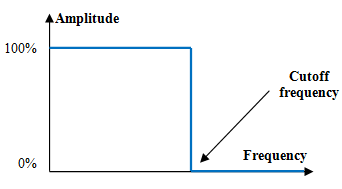
\includegraphics[width=0.4\textwidth]{images/low_pass.png}
    \caption{Low pass filter: effect of cutoff frequency on filtered measurement}
    \label{fig:low_pass}
\end{figure}

The low pass filter will be utilized to estimate the angular velocity, height, and airspeed of the UAS.
However, for the euler angles and GPS measurements, we will be using an EKF to estimate the state, as these require more complex sensor models.

The general algorithm for the EKF is given in Algorithm~\ref{alg:ekf}.

\begin{algorithm}
    \caption{Extended Kalman Filter}\label{alg:ekf}
    \begin{algorithmic}
    \State \textit{Given a system model and measurement model, predict and update the state of the system.}
    \Function{ekf}{x, P, u, z, Q, R}
    \State Predict: $\hat{x}_{k|k-1} = f(x_{k-1}, u_k)$
    \State Predict Covariance: $P_{k|k-1} = F_k P_{k-1} F_k^T + Q_k$
    \State Update: $K_k = P_{k|k-1} H_k^T (H_k P_{k|k-1} H_k^T + R_k)^{-1}$
    \State Update Estimate: $\hat{x}_k = \hat{x}_{k|k-1} + K_k (z_k - h(\hat{x}_{k|k-1}))$
    \State Update Covariance: $P_k = (I - K_k H_k) P_{k|k-1}$
    \State Return $\hat{x}_k, P_k$
    \EndFunction
    \end{algorithmic}
\end{algorithm}

The EKF works great for estimating the euler angle and GPS position measurements overtime for the UAS.
However, to estimate wind, we need to use a couple of tricks in the GPS smoothing EKF.

There is no sensor that is directly measuring the wind. But, we do have a low pass filter measuring the airspeed, $V_a$, and the GPS is able to measure the ground speed, $V_g$.
Also, we know that the way an Extended Kalman Filter works is heavily influenced by the kalman gain multiplied by the innovation. The kalman gain is the matrix $K_k$ that effectively acts as a gain for changing the estimate of the state.
The innovation is the vector $z_k - h(\hat{x}_{k|k-1})$ that represents the difference between the actual measurement, $z_k$, and the predicted measurement, $h(\hat{x}_{k|k-1})$.
Thus, the kalman gain works to drive the difference between $z_k$ and $h(\hat{x}_{k|k-1})$ to zero.

\begin{figure}[h]  
    \centering
    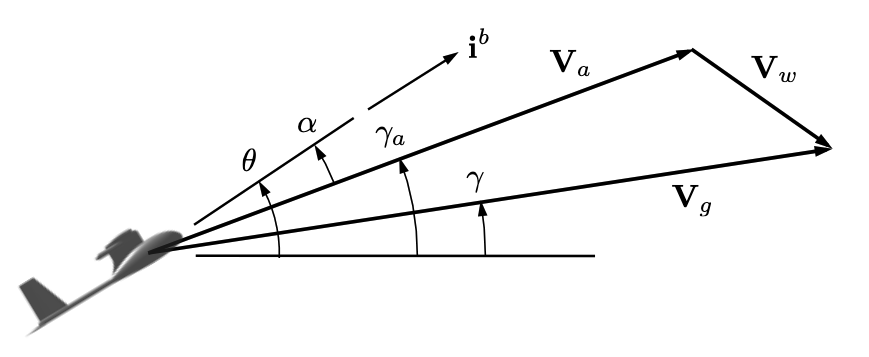
\includegraphics[width=0.4\textwidth]{images/wind_triangle.png}
    \caption{Wind triangle for a UAS, projected into the vertical plane.}
    \label{fig:wind_triangle}
\end{figure}

This concept can be exploited to estimate wind by introducting a pseudo measurement of wind.
From the wind triangle, shown in Figure~\ref{fig:wind_triangle}, we can derive the following relationships, if we assume $\gamma = \gamma_a$:

\begin{equation}
    V_a \cos(\psi) + w_n = V_g \cos(\chi)
\end{equation}
\begin{equation}
    V_a \sin(\psi) + w_e = V_g \sin(\chi)
\end{equation}

These equations can be rewritten as:
\begin{equation}
    y_{wind_n} = V_a \cos(\psi) + w_n - V_g \cos(\chi)
\end{equation}
\begin{equation}
    y_{wind_e} = V_a \sin(\psi) + w_e - V_g \sin(\chi)
\end{equation}

Therefore, we can say that we never actually estimate wind, so $z_k$ has zero value for $w_n$ and $w_e$.
But, our predicted measurement is this pseudo measurement of wind, $y_{wind_n}$ and $y_{wind_e}$.
Then, the kalman gain in the filter will choose the values of $w_n$ and $w_e$ that works to minimize the difference between $z_k$ (0s) and $h(\hat{x}_{k|k-1})$ (pseudo).
Thus, choosing the values of $w_n$ and $w_e$ that successfully completes the wind triangle with the above relationships.
This is how the EKF is able to estimate the wind in the north and east directions without every directly measuring the wind.

This results in the following state estimate for the GPS smoothing EKF:

\begin{equation}
    \hat{x}_{GPS Smoothing} = \begin{bmatrix}
        \hat{p}_{n} \\
        \hat{p}_{e} \\
        \hat{V}_{g} \\
        \hat{\chi} \\
        \hat{w}_{n} \\
        \hat{w}_{e} \\
        \hat{\psi} \\
    \end{bmatrix}
\end{equation}

While the EKF estimating the attitude measurements is simply:
\begin{equation}
    \hat{x}_{Attitude} = \begin{bmatrix}
        \hat{\phi} \\
        \hat{\theta} \\
    \end{bmatrix}
\end{equation}

From this combination of estimates from the EKF formulations along with the low pass filter estimates, the full state and wind estimate of a UAS can be filtered over time.
To see the full derivation of all matrices in the EKF, please refer to the book given in \cite{small_uas}.

\subsection{Mission Profiles and Cooperative Estimation}

% To test the impact the number of UAS has on the accuracy of the wind gradient estimation, the mission profiles tested will be a series of straight line missions.
To estimate the wind gradient for a given scenario, multiple UAS will be deployed to estimate the wind at various locations in the wind field.
Using the lookahead straight line following guidance algorithm, we will simulate multiple UAS flying in a stacked formation.
A stacked formation is a formation where the UAS are flying at straight level paths through the wind field, but at different altitudes. 
This is shown in Figure~\ref{fig:stacked_formation}.

\begin{figure}[h]  
    \centering
    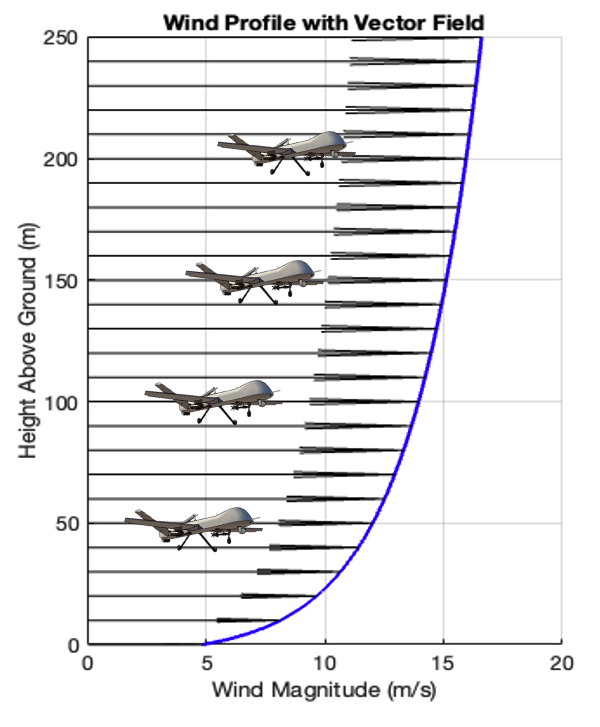
\includegraphics[width=0.4\textwidth]{images/stacked.png}
    \caption{Stacked UAS formation for estimating wind gradient.}
    \label{fig:stacked_formation}
\end{figure}



It is assumed to collabratively estimate the wind gradient, each UAS has the ability to communicate back to some centralized location; likely a ground station.
This ground station will then have online access to the state and wind estimates of all UAS at a given time step. 
Using these measurements, the wind gradient parameters $a$ and $b$ can be estimated.
